\title{Study Guide for Midterm 2}
\author{Dr. Jordan Hanson - Whittier College Dept. of Physics and Astronomy}
\date{\today}
\documentclass[10pt]{article}
\usepackage[a4paper, total={18cm, 27cm}]{geometry}
\usepackage{outlines}
\usepackage{graphicx}
\usepackage{diagbox}
\usepackage{tcolorbox}

\begin{document}
\maketitle

\section{Chapter 5 - Combinatorial Logic Analysis}
\label{sec:comb}

\begin{figure}[ht]
\centering
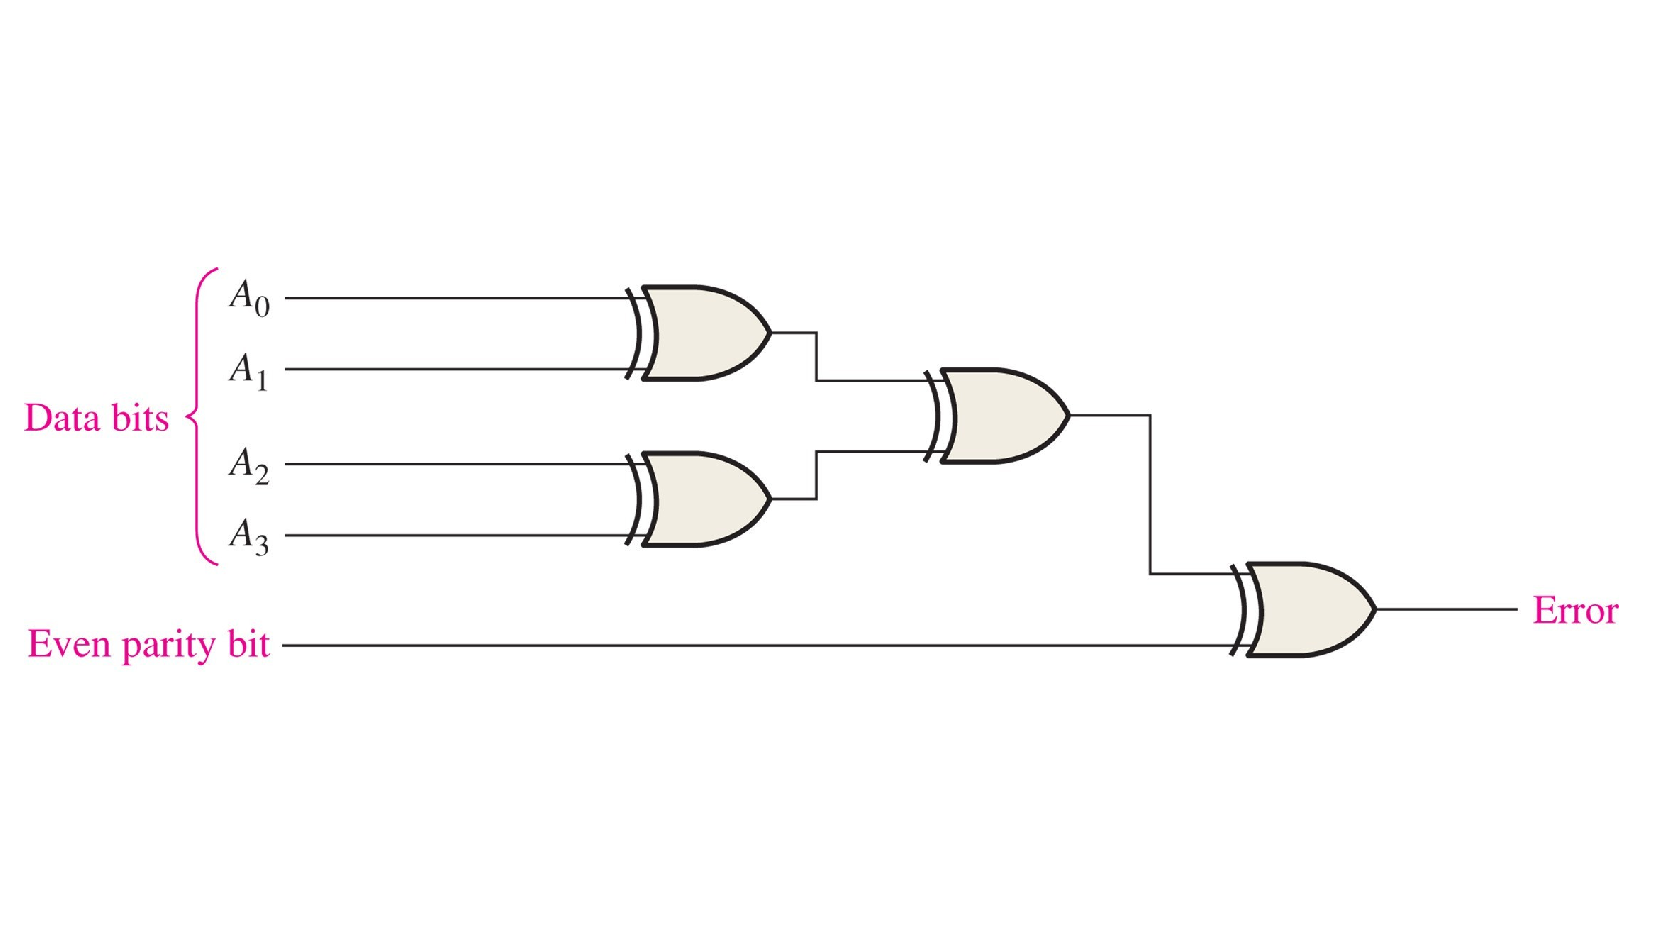
\includegraphics[width=0.45\textwidth,trim=0cm 4cm 0cm 4cm,clip=true]{figures/parityCheck.pdf} \hspace{0.25cm}
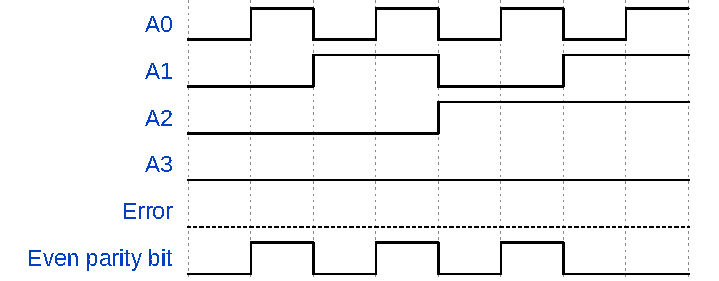
\includegraphics[width=0.4\textwidth]{figures/timingExample9.pdf}
\caption{\label{fig:par} (Left) A circuit involving several XOR gates. (Right) An example timing diagram for the circuit at left.}
\end{figure}

\begin{enumerate}
\item Consider Fig. \ref{fig:par}.  (a) Generate the truth table for the output of the first three XOR gates, for all possible values of the 4-bit binar	y input.  What does this output represent numerically about the input $\vec{A}$? (b) Fill in the Error bit stream in Fig. \ref{fig:par}. \\
\begin{table}[ht]
\centering
\begin{tabular}{| c | c | c | c | c |}
\hline
$A_3$ & $A_2$ & $A_1$ & $A_0$ & input to parity XOR \\ \hline \hline
0 & 0 & 0 & 0 & 0 \\ \hline
0 & 0 & 0 & 1 & 1 \\ \hline
0 & 0 & 1 & 0 & 1 \\ \hline
0 & 0 & 1 & 1 & 0 \\ \hline
0 & 1 & 0 & 0 & 1 \\ \hline
0 & 1 & 0 & 1 & 0 \\ \hline
0 & 1 & 1 & 0 & 0 \\ \hline
0 & 1 & 1 & 1 & 1 \\ \hline
1 & 0 & 0 & 0 & 1 \\ \hline
1 & 0 & 0 & 1 & 0 \\ \hline
1 & 0 & 1 & 0 & 0 \\ \hline
1 & 0 & 1 & 1 & 1 \\ \hline
1 & 1 & 0 & 0 & 0 \\ \hline
1 & 1 & 0 & 1 & 1 \\ \hline
1 & 1 & 1 & 0 & 1 \\ \hline
1 & 1 & 1 & 1 & 0 \\ \hline
\end{tabular}
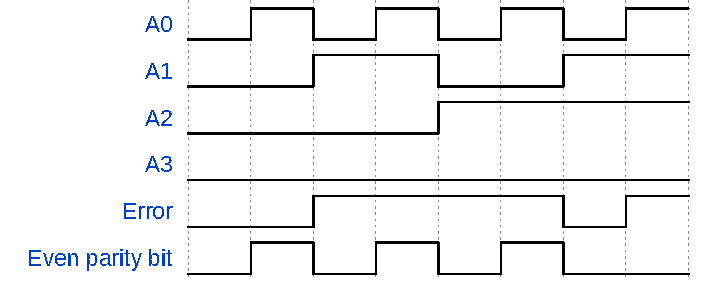
\includegraphics[width=0.5\textwidth]{figures/timingExample10.pdf}
\caption{\label{tab:par} (Left) The output of the first three XOR gates yields the \textit{parity}: true if the input contains an odd number of 1's. (Right) Fig. \ref{fig:par} with the error line completed.}
\end{table}
\clearpage
\item In Fig. \ref{fig:gates1}, (a) simplify the circuit via the Karnaugh map. (b) For the resulting domain-2 logic function, connect $A0$ and $A1$ from Fig. \ref{sec:comb} (right) as inputs and produce the timing diagram assuming the same even parity bit stream. \\
\begin{table}
\centering
\begin{tabular}{| c | c | c | c | c |}
\hline
\backslashbox{AB}{CD} & 00 & 01 & 11 & 10 \\ \hline
00 & 0 & 1 & 1 & 0 \\ \hline
01 & 0 & 0 & 0 & 0 \\ \hline
11 & 0 & 0 & 0 & 0 \\ \hline
10 & 0 & 1 & 1 & 0 \\ \hline
\end{tabular}

\includegraphics[width=0.35\textwidth]{figures/gateExample7.pdf} \\ \vspace{0.5cm}
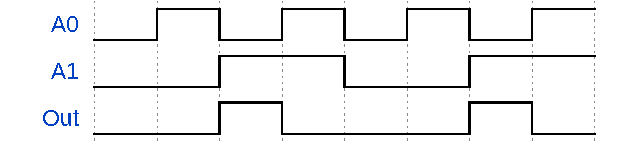
\includegraphics[width=0.35\textwidth]{figures/timingExample11.pdf}
\caption{\label{tab:Kmap1} The Karnaugh map for the circuit in Fig. \ref{fig:gates1}.}
\end{table}

The domain-4 Karnaugh map is shown in Tab. \ref{tab:Kmap1} (left), and the simplified circuit in Tab. \ref{tab:Kmap1} (right).  The gate structure only has two inputs because there are 4 adjacent cells in Tab. \ref{tab:Kmap1} (left).  The parity bit stream is irrelevant because there are only two inputs.  The correct output for the simplified gate is shown in Tab. \ref{tab:Kmap1} (bottom).

\end{enumerate}

\begin{figure}[hb]
\centering
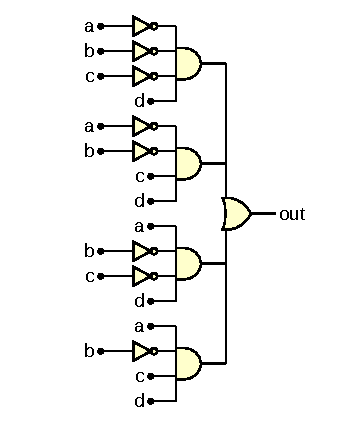
\includegraphics[width=0.3\textwidth]{figures/gateExample6.pdf}
\caption{\label{fig:gates1} A domain-4 logic function.}
\end{figure}



\section{Chapter 6 - Functions of Combinational Logic}
\label{sec:comb2}

\begin{figure}[ht]
\centering
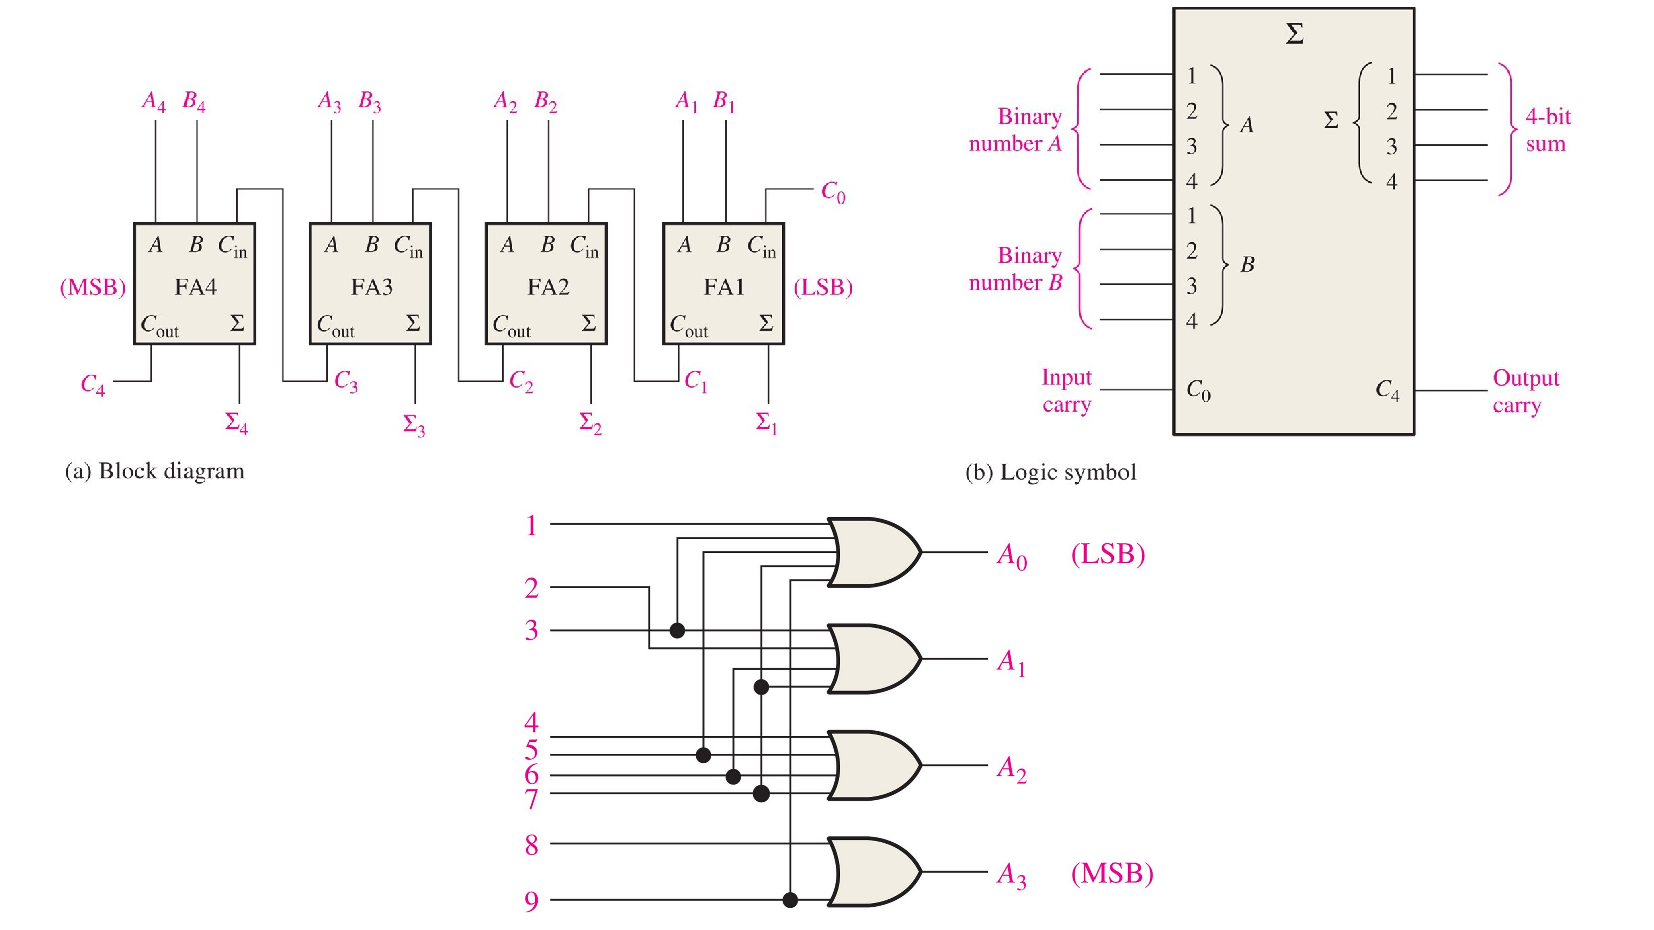
\includegraphics[width=0.6\textwidth]{figures/adderEncoder.pdf}
\caption{\label{fig:encadd} A 4-bit ripple carry adder (with logic symbol), and a 9-digit (zero ommitted) encoder.}
\end{figure}

\begin{enumerate}
\item Consider Fig. \ref{fig:encadd}.  (a) Design a circuit below that adds two numbers in binary corresponding to outputs from two separate encoders. (b) Demonstrate how your design would add 1 and 9.  (c) Add a separate input line with XNOR gates that switches the system to subtraction in 2's complement form. \\

\begin{figure}[ht]
\centering
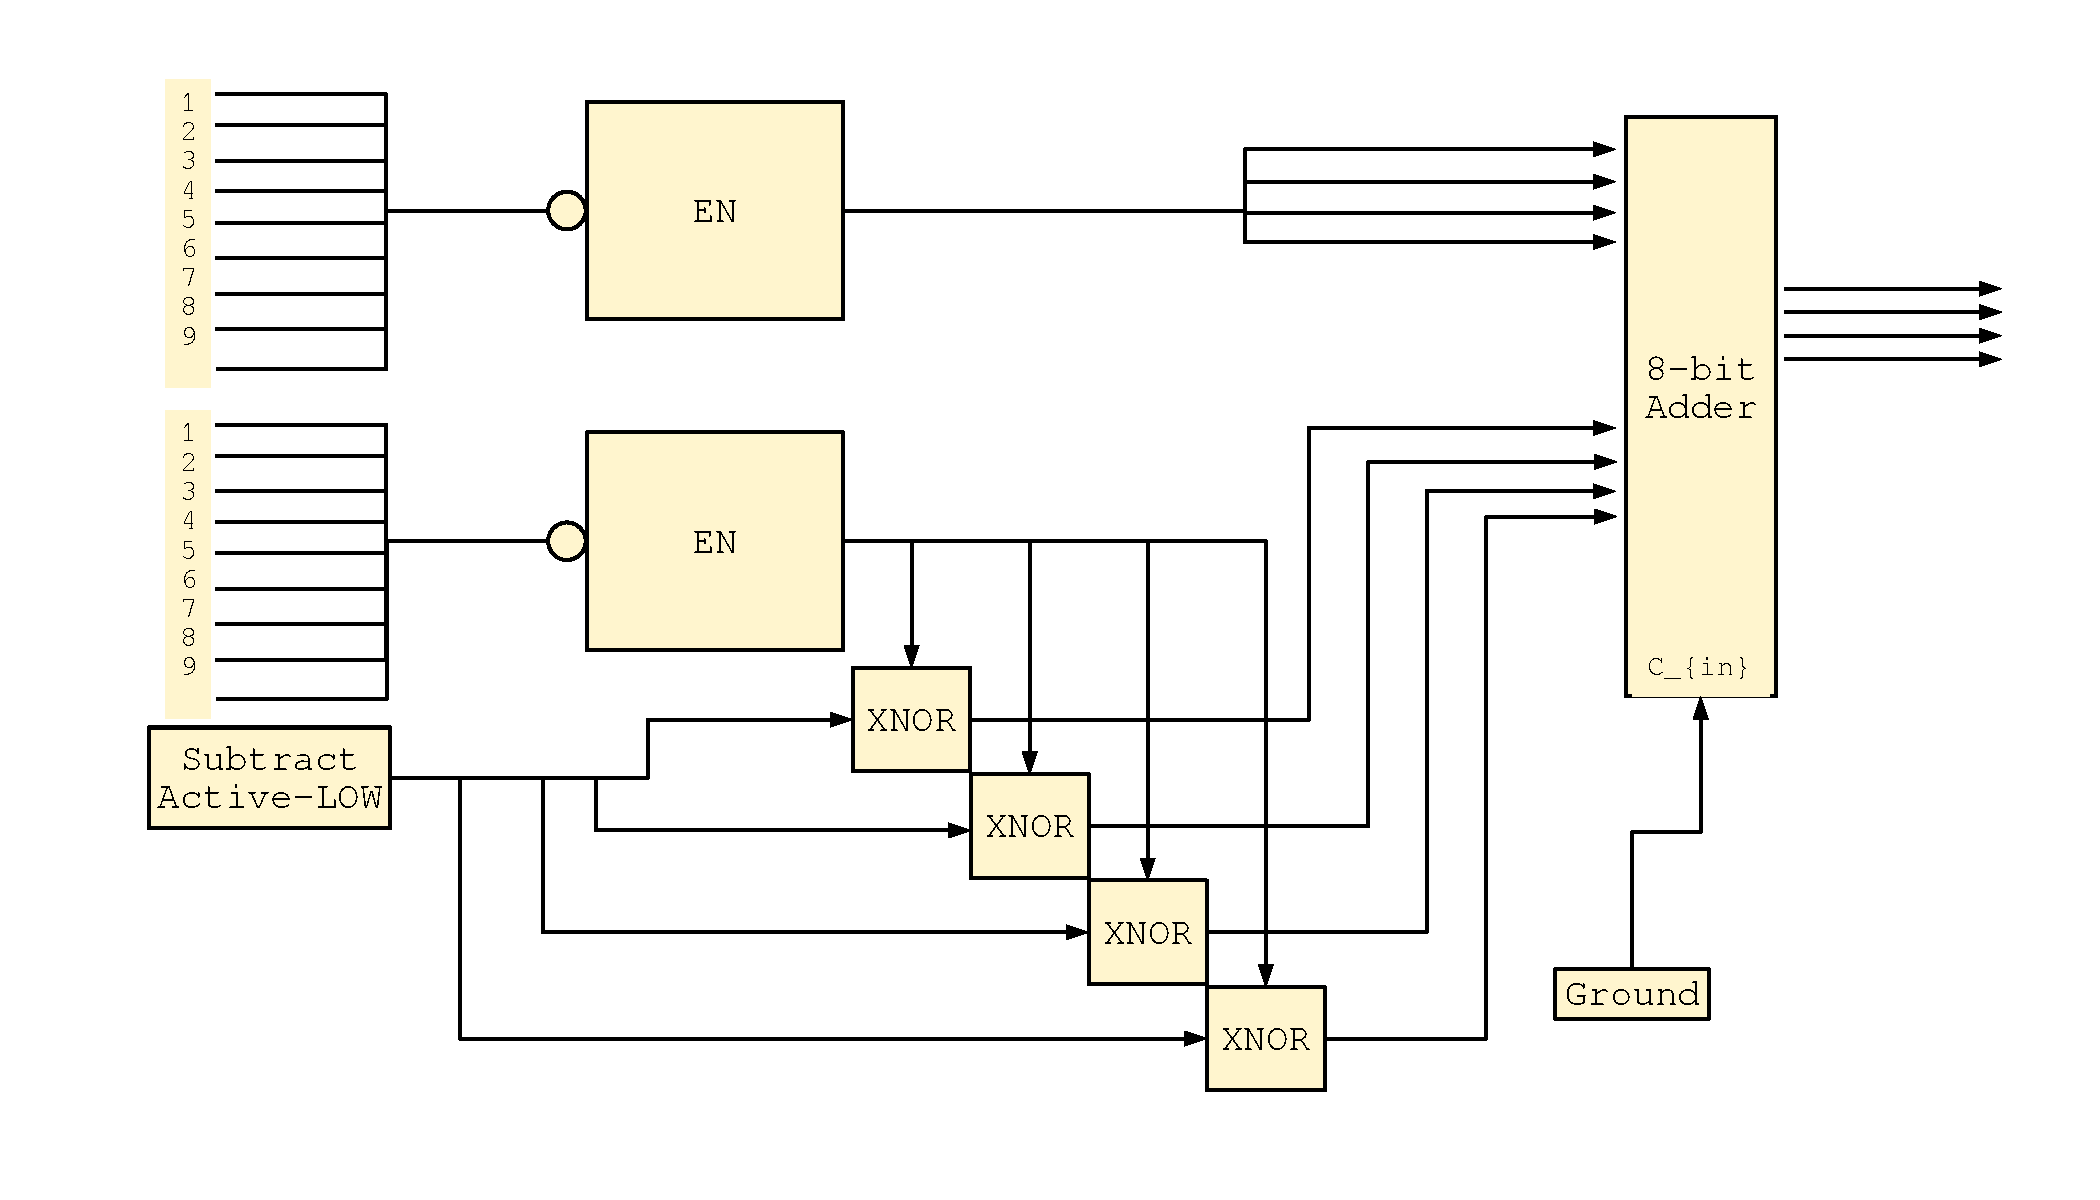
\includegraphics[width=0.8\textwidth]{figures/design1.pdf}
\caption{\label{fig:design1} The system adds two active-LOW key presses 1-9 (0 is default) by passing them to two BCD encoders.  The active-LOW negative sign switch converts the second digit to the 1's complement via the XNOR gate array.}
\end{figure}

(a) See Fig. \ref{fig:design1}.  (b) If the 1 key is pressed on the upper pad, then 1 is encoded to 0001 in the encoder.  If the 9 key is pressed on the lower pad, the encoder converts to 1001.  If the subtract key is not pressed, then it remains HIGH and the outputs of the XNOR gates follow the outputs of the bottom encoder.  The outputs of the two encoders are fed to the four pairs of inputs to the 8-bit adder with carry-in tied to ground.  The result is the output of the 8-bit addition of 1001 and 0001, or 1010. (c) If the subtract key is pressed, the active-LOW signal pulls down one input on each of the XNOR gates, making the XNOR outputs the complements of the bottom encoder.  Instead of connecting $C_{in}$ to ground, we would connect it to the complement of the subtract signal (via an inverter).

\clearpage

\item Using the basic logic in Fig. \ref{fig:2bit}, plus inverters, (a) create a circuit that compares the \textit{magnitude} of two 2-bit binary numbers.  Assume that one or both of the numbers is a negative one, and that if a number is negative it is in \textit{1's complement form.} \\ 
\begin{figure}[ht]
\centering
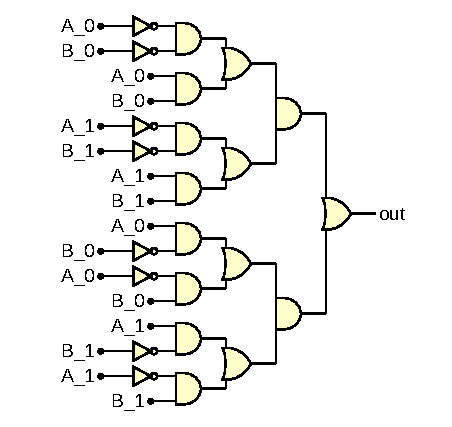
\includegraphics[width=0.5\textwidth]{figures/gateExample8.pdf}
\caption{\label{fig:comp1} A comparator that compares the magnitude of a pair of 2-bit binary numbers.  There are two top-level AND gates.  The upper AND gate has two XNOR gates comparing $A$ and $B$.  The lower AND gate has two XNOR gates comparing $\bar{A}$ and $B$.}
\end{figure}
\item For the first four binary numbers (0, 1, 2, 3) show that the logic in Fig. \ref{fig:2bit} (right) converts binary to gray code. \\

See Tab. \ref{tab:gray}.

\begin{table}[hb]
\centering
\begin{tabular}{| c | c |}
\hline
Input & Output \\ \hline \hline
000 & 000 \\ \hline
001 & 001 \\ \hline
010 & 011 \\ \hline
011 & 010 \\ \hline
\end{tabular}
\caption{\label{tab:gray} Verification that Fig. \ref{fig:2bit} (right) contains the gray-code converter from binary.}
\end{table}
\end{enumerate}

\begin{figure}[hb]
\centering
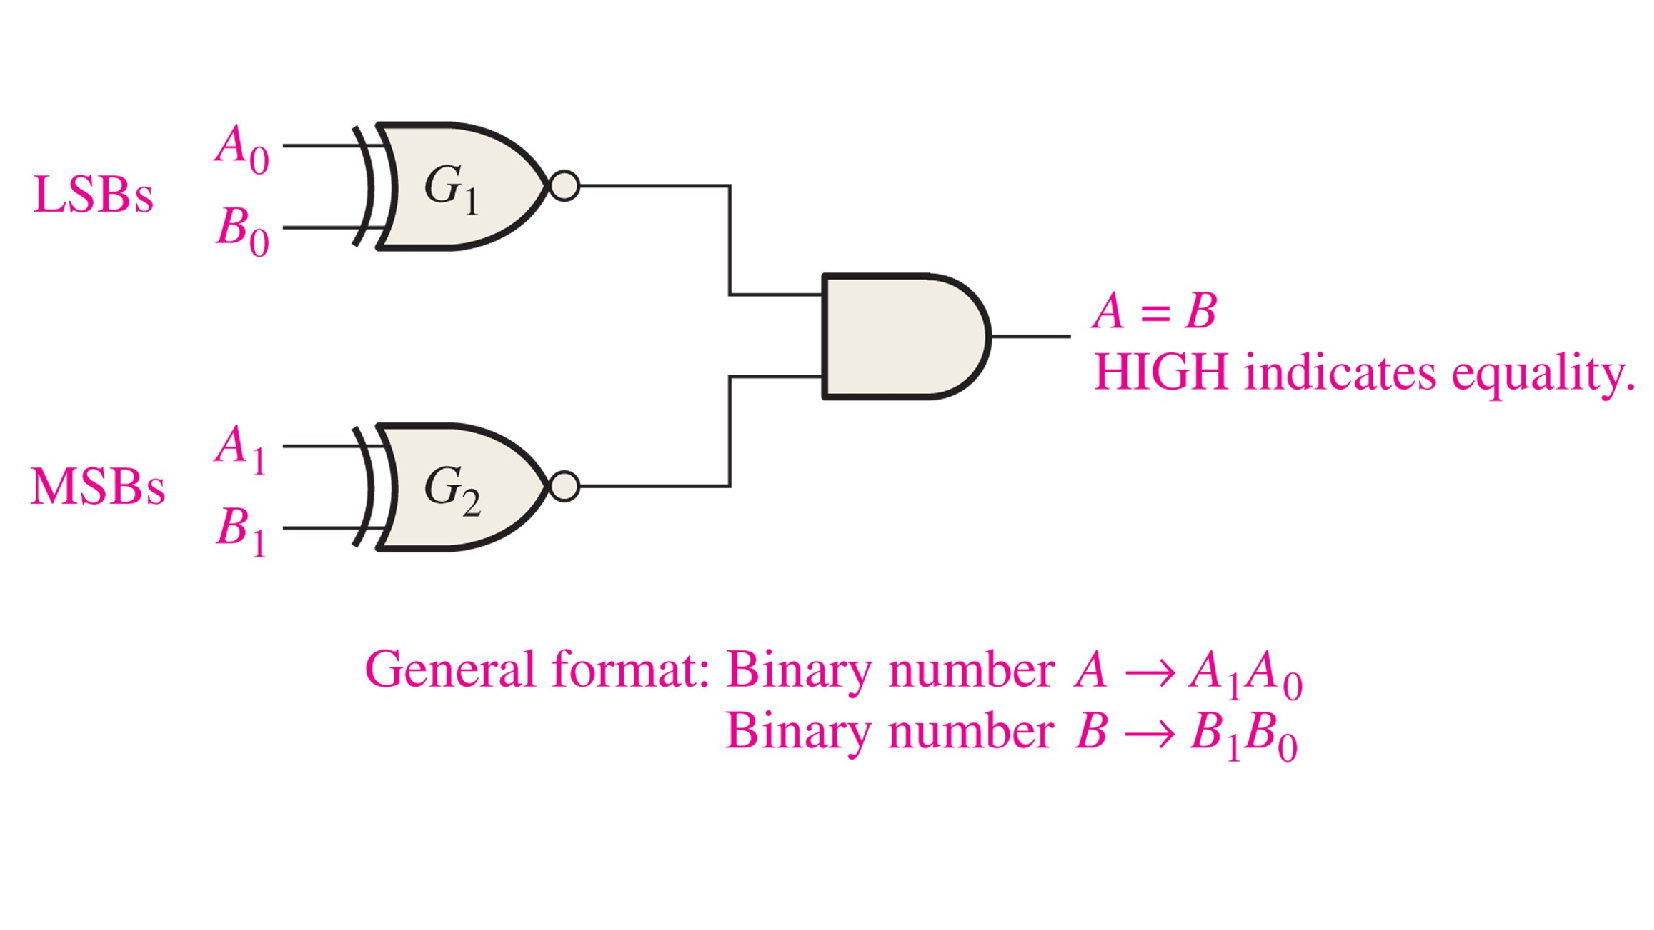
\includegraphics[width=0.4\textwidth]{figures/2bitcomparator.pdf} \hspace{0.25cm}
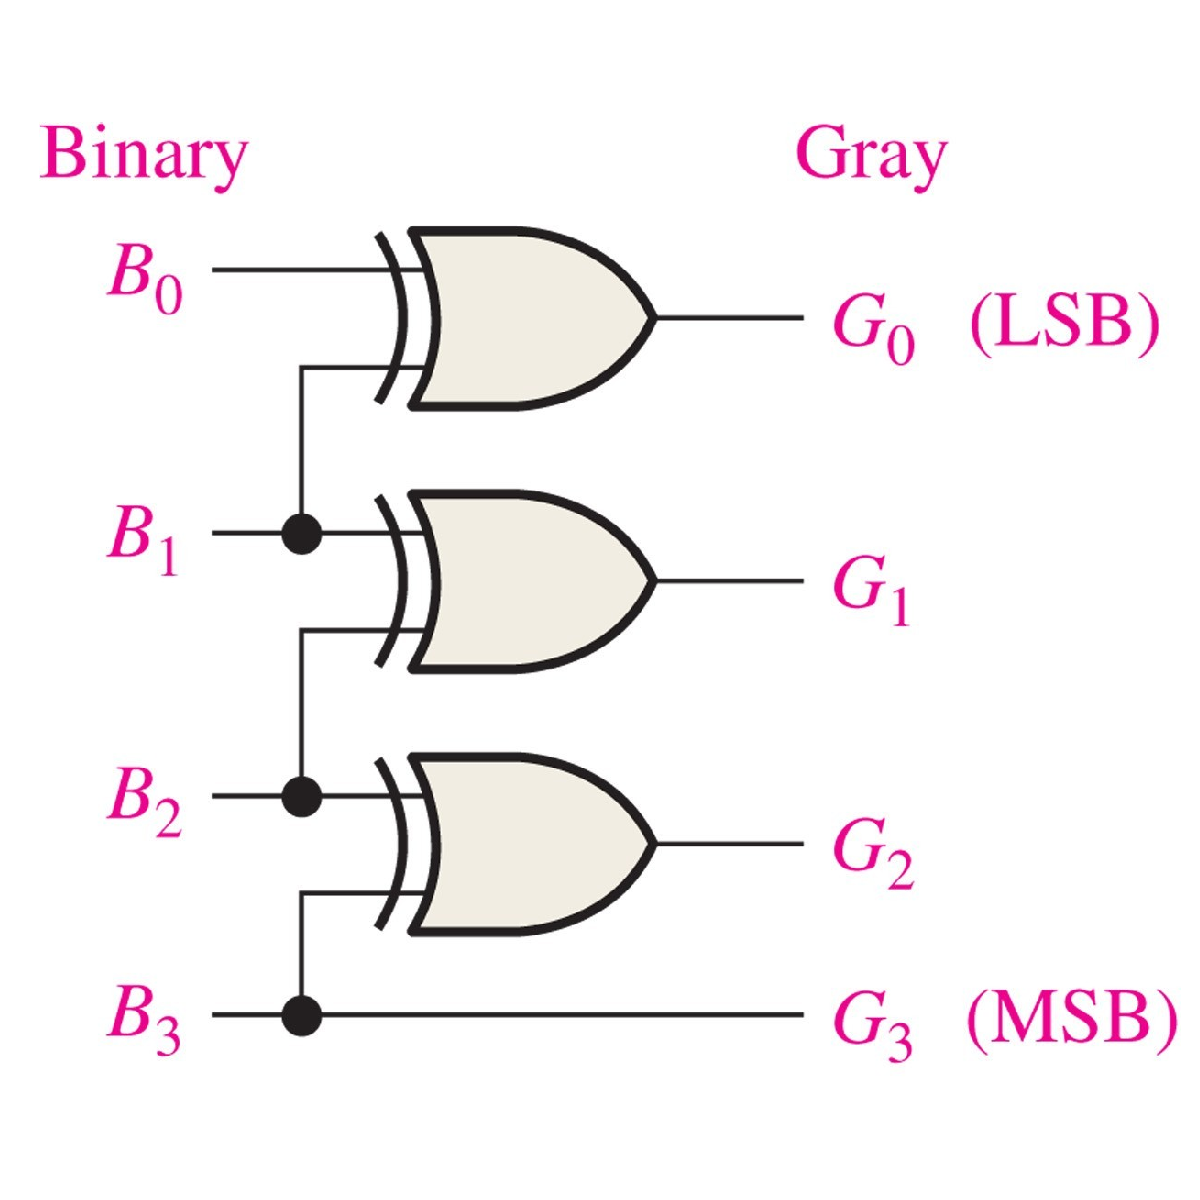
\includegraphics[width=0.25\textwidth]{figures/binaryGray.pdf}
\caption{\label{fig:2bit} (Left) This is how a 2-bit comparator works. (Right) A binary to gray code converter.}
\end{figure}

\clearpage

\section{Chapter 7 - Latches, Flip-flops, and Timers}
\label{sec:latch}

\begin{figure}[ht]
\centering
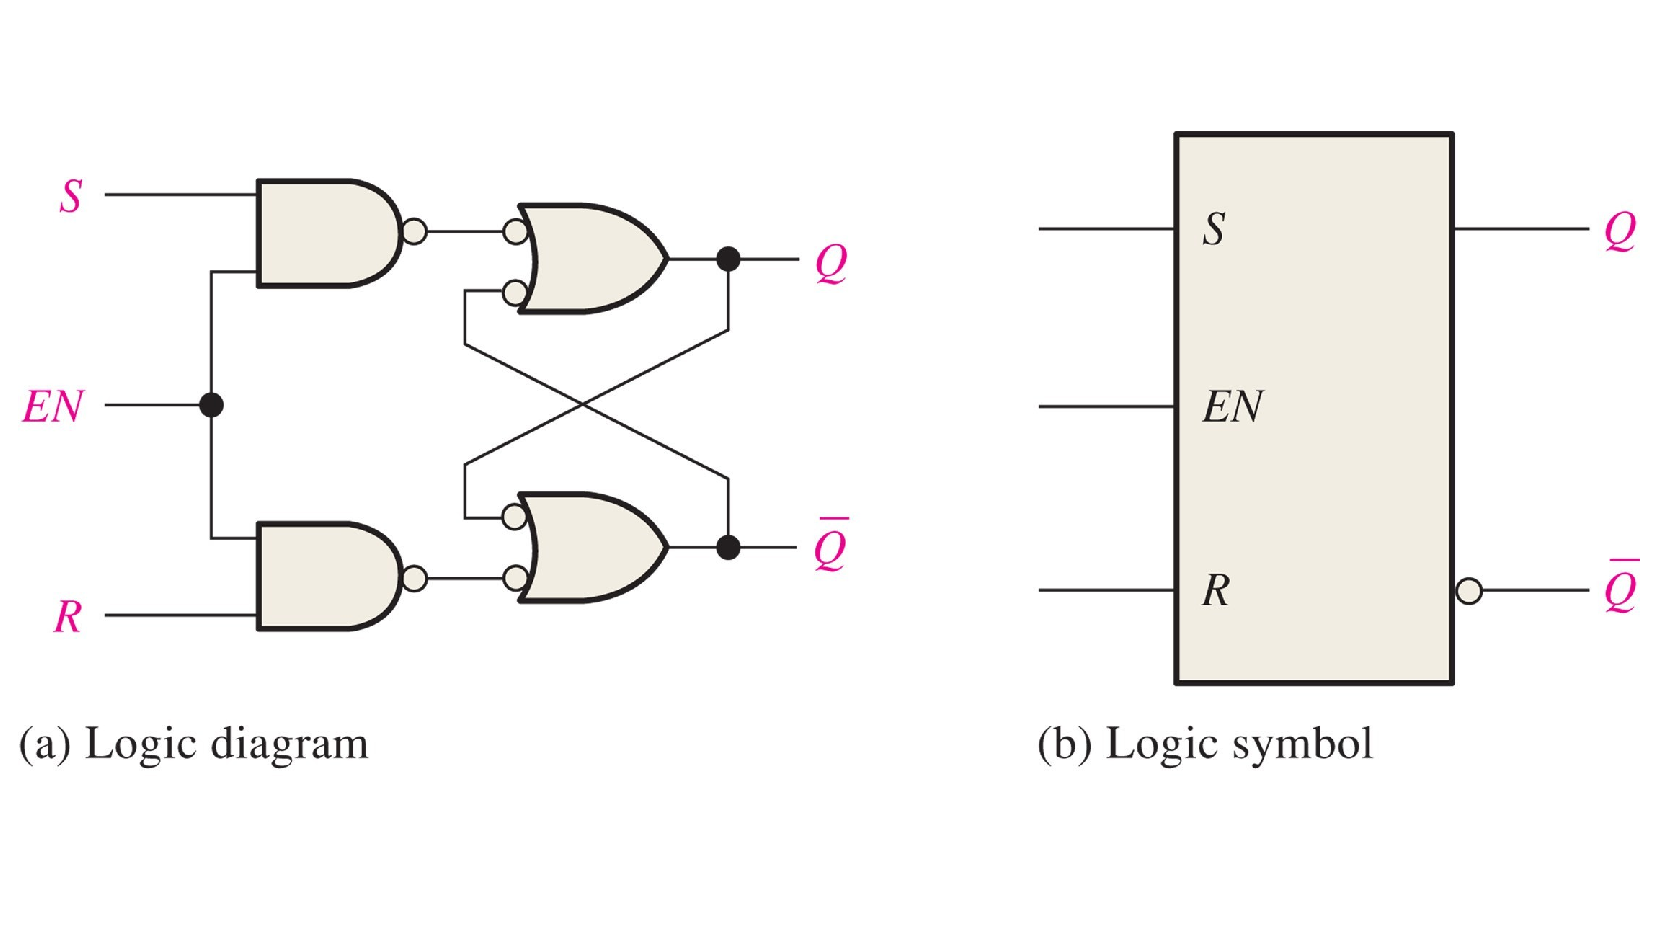
\includegraphics[width=0.5\textwidth]{figures/enSRLatch.pdf} \hspace{0.5cm}
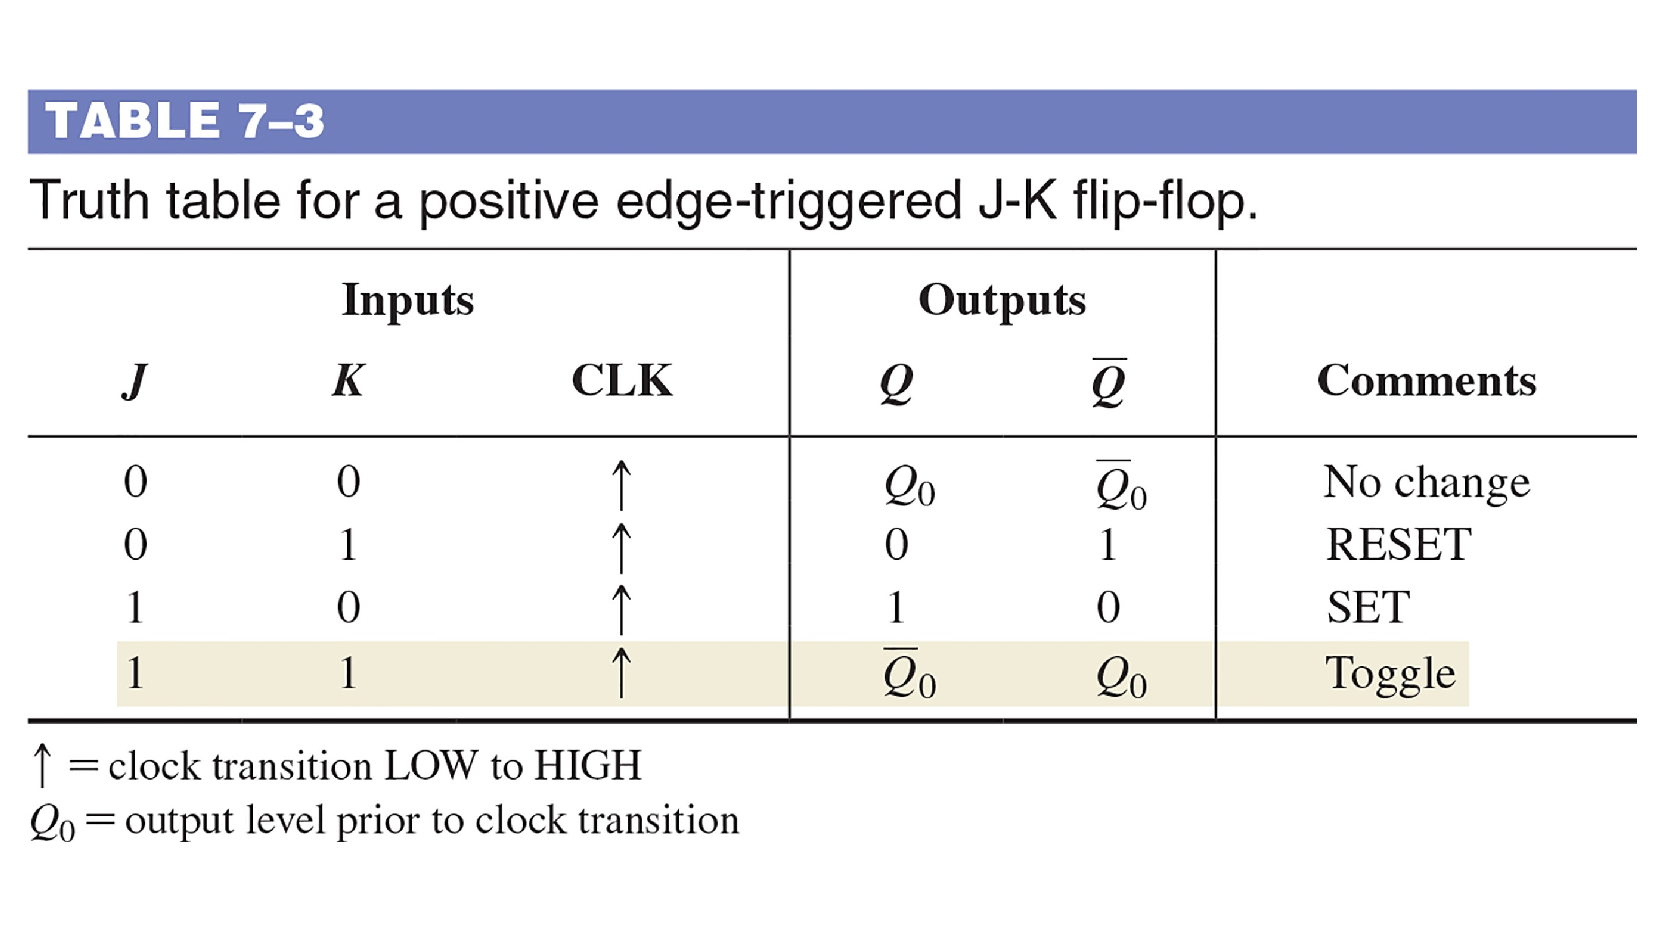
\includegraphics[width=0.5\textwidth]{figures/jkFlopTT.pdf}
\caption{\label{fig:latch} (Top) The gate-enabled SR latch. (Bottom) The truth table for the JK flip-flop.}
\end{figure}

\begin{enumerate}
\item Using the logic for the gate-enabled SR latch in Fig. \ref{fig:latch} (top), develop a system that (a) activates a green LED when the circuit is enabled and in SET mode, (b) a yellow LED switch when the circuit is enabled and in RESET mode, and (c) a red LED when the circuit is not enabled. \\

See Fig. \ref{fig:latchDesign} (left).  The red LED is pulled low with a LOW on the enable input.  When Q is SET, the LED is on, and when the complement of Q is RESET, the yellow LED is on.  Q and its complement are never high simultaneously.

\begin{figure}[hb]
\centering
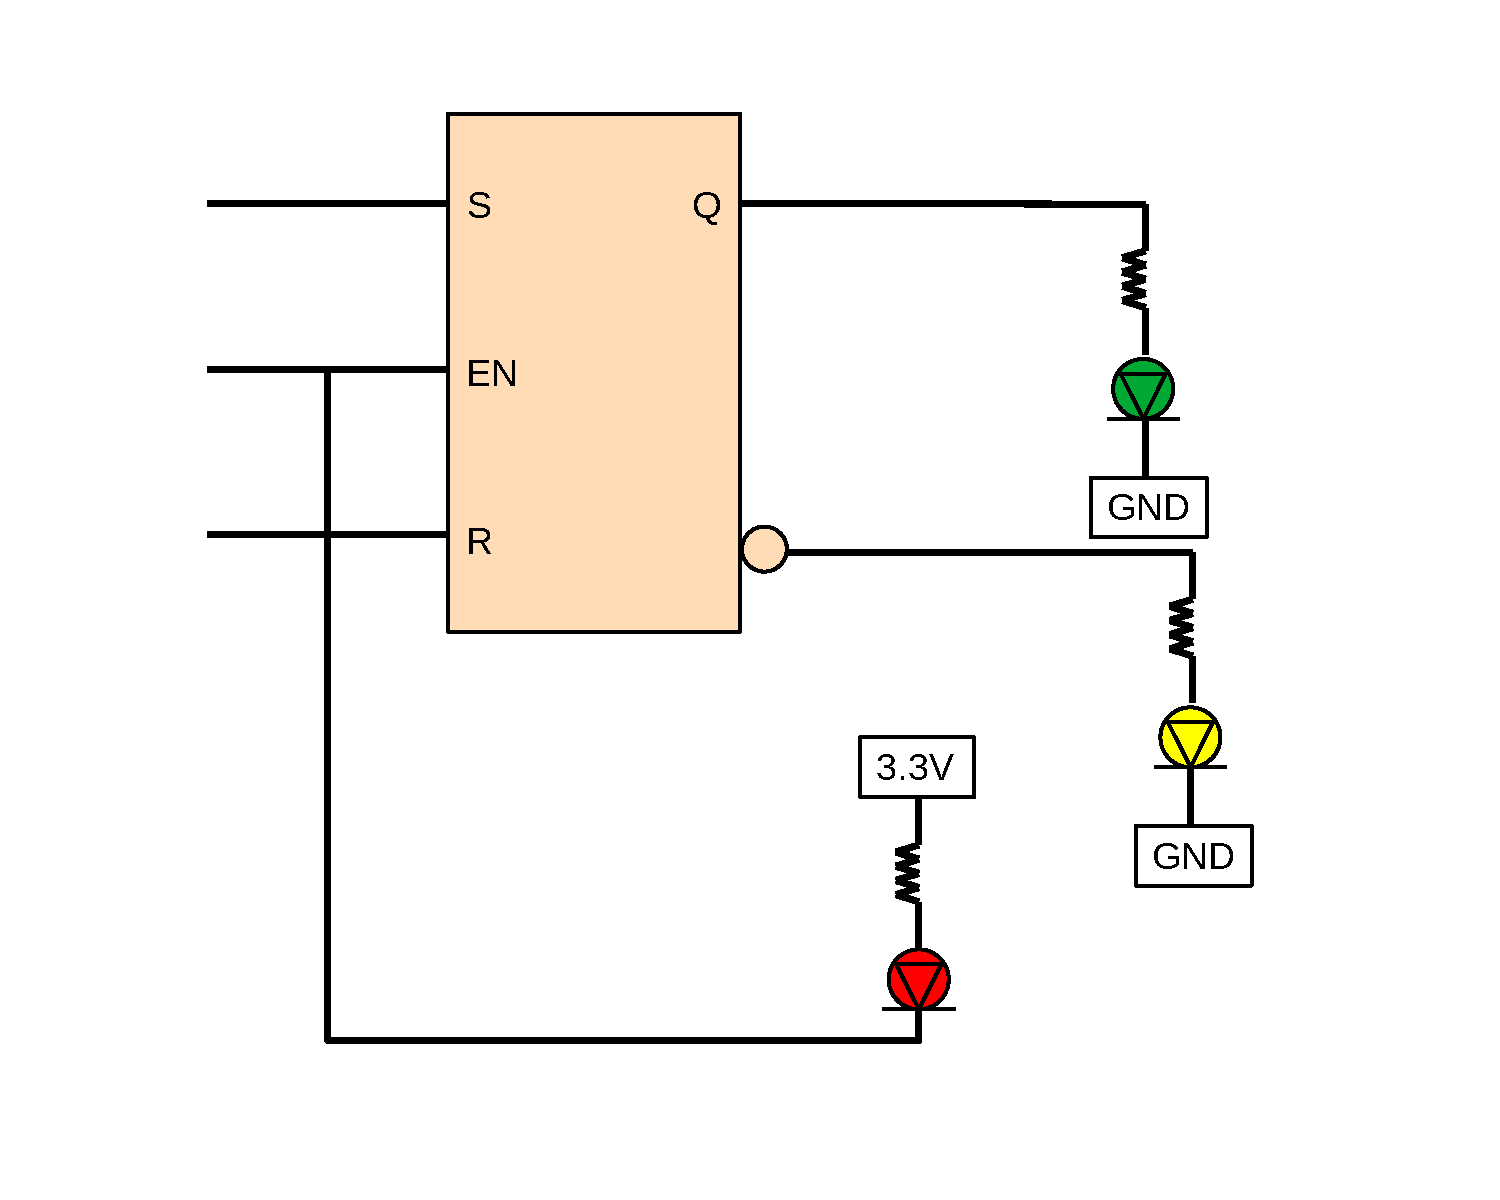
\includegraphics[width=0.4\textwidth]{figures/design2.pdf} \hspace{0.5cm}
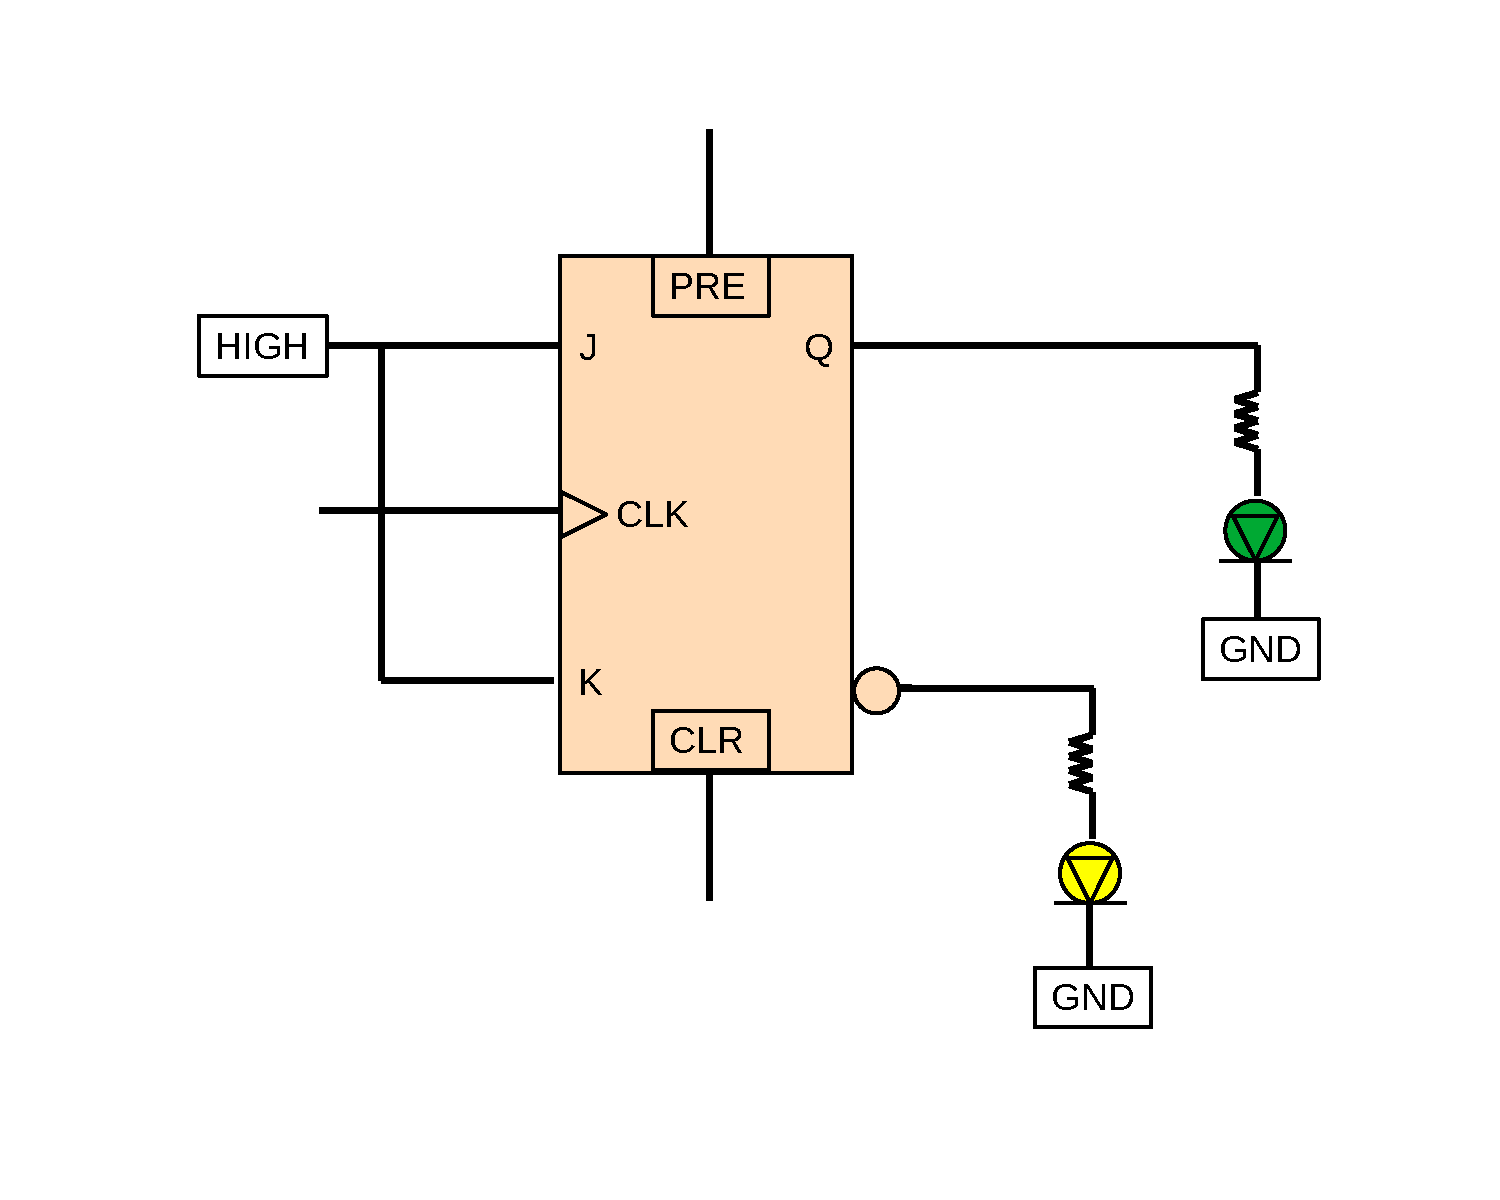
\includegraphics[width=0.4\textwidth]{figures/design3.pdf}
\caption{\label{fig:latchDesign} (Left) Remember that the gate-enabled SR latch shown in Fig. \ref{fig:latch} is an active-HIGH design. (Right) The posedge-triggered JK flip-flop with preset and clear functions toggling two LEDs.}
\end{figure}
\item The truth table for a positive clock-edge JK flip-flop is shown in Fig. \ref{fig:latch} (bottom).  Use such a device to design a circuit below that (a) powers two LEDs, and toggles between two states: one in which one LED is activated, and another in which the opposite LED is activated. The lights should switch on positive edges of the clock.  (b) Add logic that holds LED1 on, and LED2 off, regardless of the outputs of the JK flip-flop (the equivalent of \textit{preset} and \textit{clear} functions of JK flip-flops). \\

See Fig. \ref{fig:latchDesign} (right).  The key is that the J and K inputs are tied together so that the LEDs are always toggled on posedge. Preset and clear active-LOW would hold one or the other LED on regardless of J and K.
\end{enumerate}

\end{document}